% !TeX spellcheck = en_GB
\section{Verification}
In this section we present tests performed in order to verify that our implementation reflects correctly our model.

\subsection{Degeneracy Tests}
In the degeneracy tests we verify the behaviour of our simulator with parameters set to 0 values. In all tests the simulator works properly. In particular the following observations can be inferred:
\begin{itemize}
	\item If the number of channel is 0 then the simulation stops immediately because has no sense running a simulation with 0 channels.
	\item If the time slot size is 0 then the simulation doesn't stop and goes to infinite because on instant 0  time slots are continuously triggered.
	\item If the exponential mean is 0 then the simulation doesn't stop and continues to infinite because packets arrive at time 0 continuously.
\end{itemize}

\subsection{Consistency Test}
The consistency test verifies that the system react consistently with the output. In order to test this we perform two tests with the following parameters.
\paragraph{Test 1}
\begin{itemize}
	\item Number of couple tx-rx: 1
	\item Number of channels: 500
	\item Send probability: 1
	\item Mean inter-arrival time: 10s (deterministic)
	\item Time slot size: 5s
\end{itemize}

\paragraph{Test 2: Two couple TX-RX with half packets arrival rate}
\begin{itemize}
	\item Number of couple tx-rx: 2
	\item Number of channels: 500
	\item Send probability: 1
	\item Mean inter-arrival time: 20s (deterministic)
	\item Time slot size: 5s
\end{itemize}

\noindent We expect that the result of the two tests are more or less equal because the behaviour of one source transmitting every 10 seconds must be similar to the behaviour of two sources transmitting every 20 seconds. We set the number of channels at 500 in order to neglect the effect of collisions (in any case it is possible that a collision occur, but in the following tests no collisions have been detected).

\noindent The graph in figure \ref{img: consistencyTest1a} and in figure \ref{img: consistencyTest1b} show the results of the tests previously explained. We can see that the behaviour is very similar in both cases and so that the systems works as we expect. In fact the Mean Throughput per slot tend in both cases to 0.50 packets per slot.

\begin{figure}[H]
	\centering
	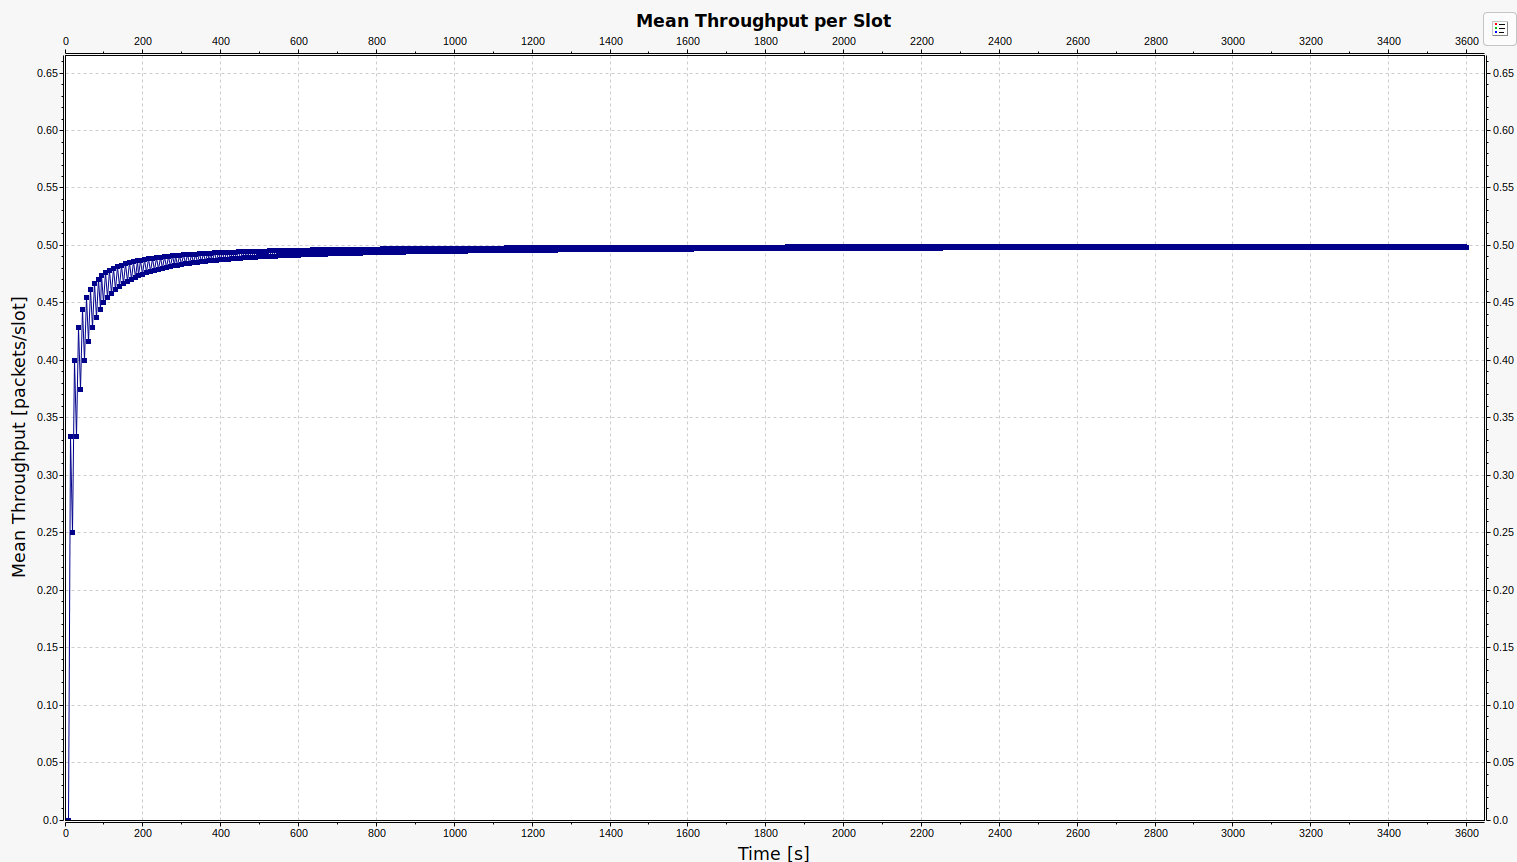
\includegraphics[width=0.9\textwidth]{img/consistencyTest1aWithAxis.png}
	\caption{Consistency Test 1}
	\label {img: consistencyTest1a}
\end{figure}

\begin{figure}[H]
	\centering
	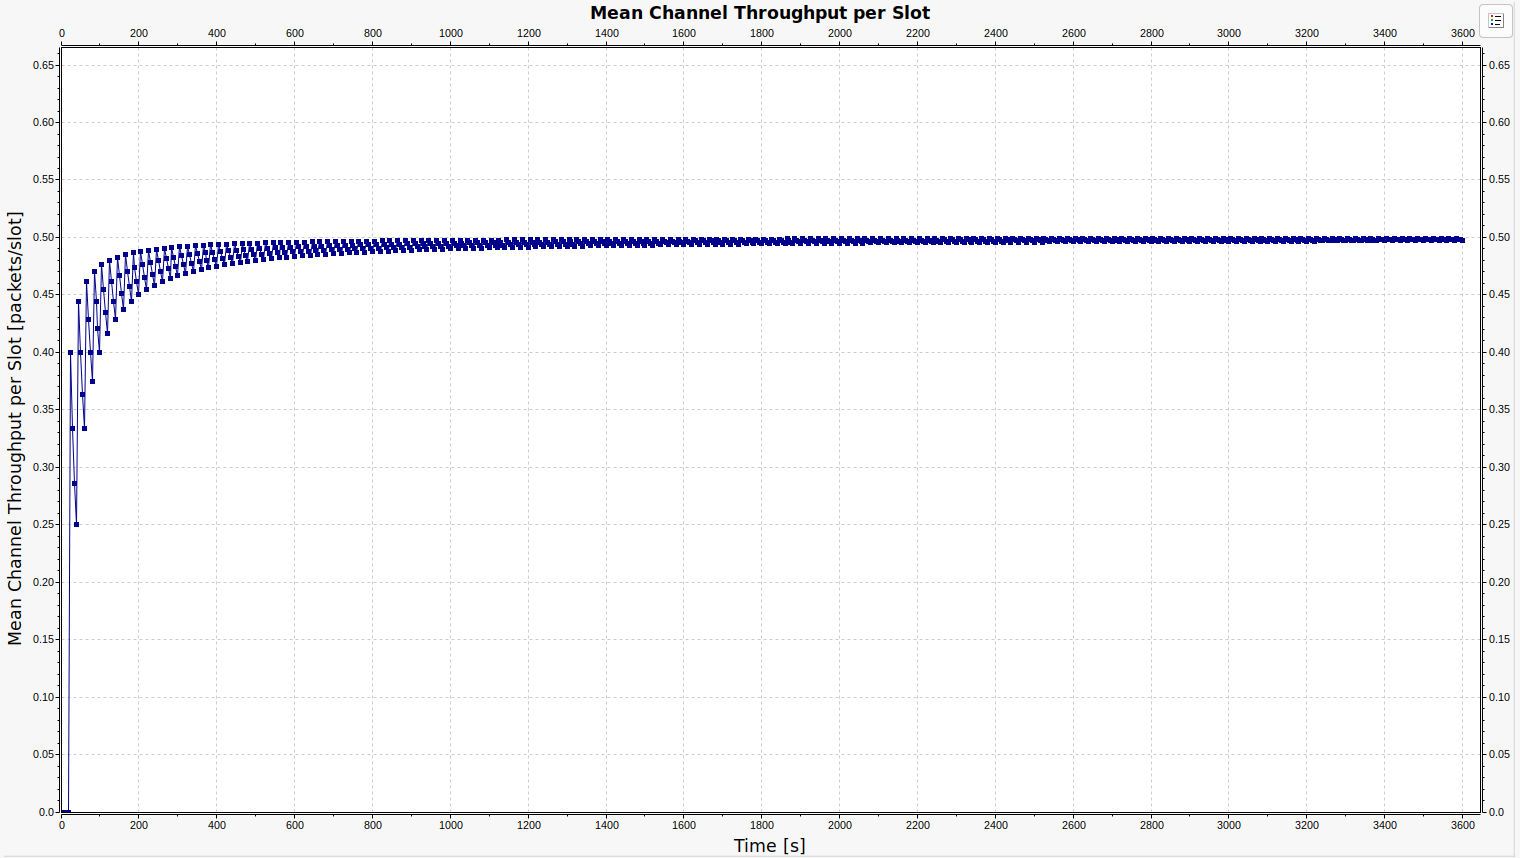
\includegraphics[width=0.9\textwidth]{img/consistencyTest1bWithAxis.png}
	\caption{Consistency Test 2}
	\label {img: consistencyTest1b}
\end{figure}

\noindent The oscillations at the beginning are due to the fact that the mean inter-arrival time is bigger with respect to the time slot size. In fact we can observe that in the second test there are larger oscillations because the difference between the mean inter-arrival time and the time slot size is bigger than the one of the first test.

\noindent Now let analyse the response time, we can see its measure in both tests in figure \ref{img: consistencyTest1a_responsetime} and \ref{img: consistencyTest1b_responsetime}.

\begin{figure}[H]
	\centering
	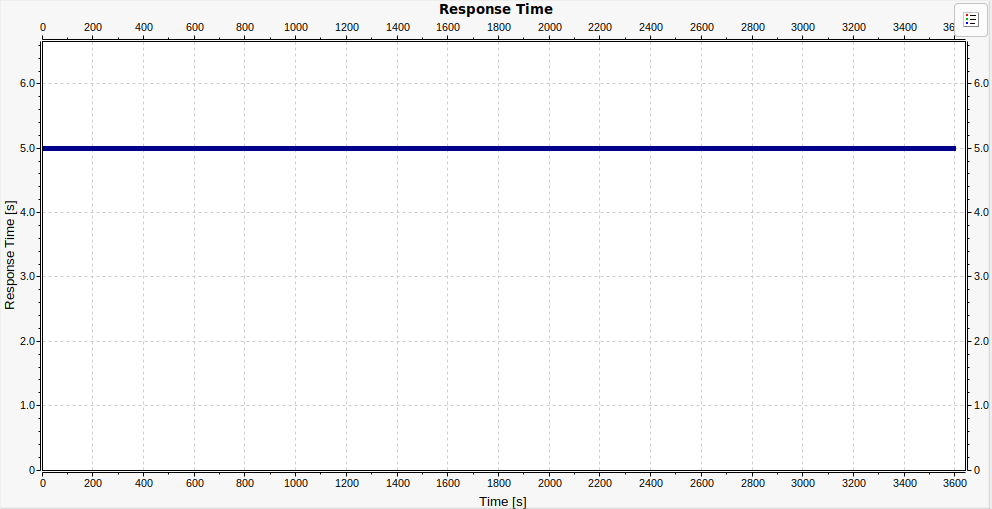
\includegraphics[width=0.9\textwidth]{img/consistencytest1a_responsetime.png}
	\caption{Consistency Test 2 - Response Time}
	\label {img: consistencyTest1a_responsetime}
\end{figure}

\begin{figure}[H]
	\centering
	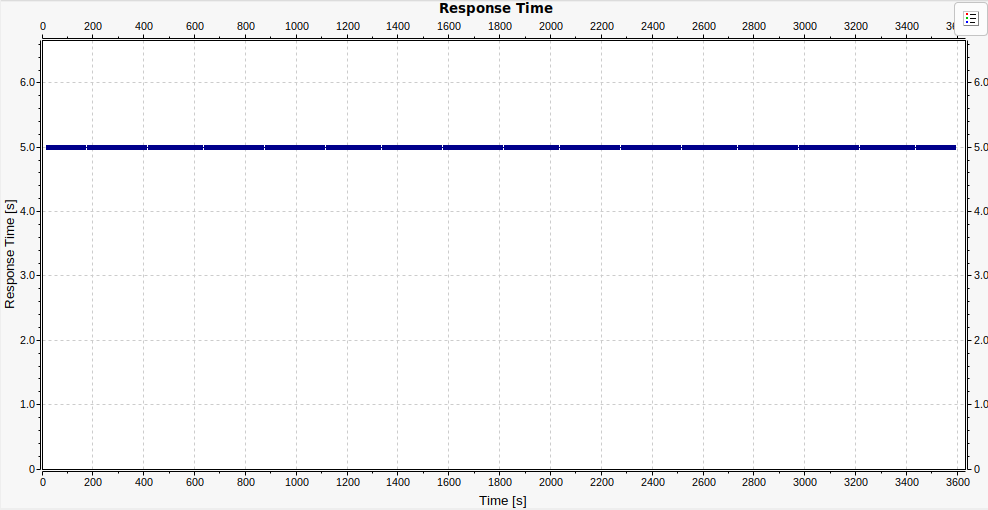
\includegraphics[width=0.9\textwidth]{img/consistencytest1b_responsetime.png}
	\caption{Consistency Test 2 - Response Time}
	\label {img: consistencyTest1b_responsetime}
\end{figure}


\noindent The mean response time in both cases is 5 seconds, this is a lower bound for the response time because in both tests 5 seconds is the size of the slot time so it's impossible to have a response time lower than the slot size.

\noindent We can see that in the second test we have a less continue plot, this is due to the fact that the mean inter-arrival time is bigger in the second case and so the packet are more distant in time.

\noindent We can conclude that also for what concerns the response time the consistency is ensured because it is the same in the case in which we have a source transmitting each 10 seconds and in the case in which we have two sources transmitting each 20 seconds. 

\subsection{Continuity Test}
In this test the aim is to prove that the output changes slightly if the input changes a bit. In order to do prove this, 2 simulations have been performed with the parameters shown in table \ref{tab: continuity test}. With this parameters we have changed slightly the input, and so we expect that the outputs don't show particular differences. Obviously some differences will be present (in particular due to collisions and the increasing in the number of transmitters) but they shouldn't affect a lot the results.

\begin{table}[htpb]
	\centering
		\begin{tabular}{|c|c|c|ll}
			\cline{1-3}
			{\textbf{Test}} & { \textbf{Number of Transmitters}} & { \textbf{Number of Channels}} &  &  \\ \cline{1-3}
			1 & 8  & 20 &  &  \\ \cline{1-3}
			2 & 10 & 20 &  &  \\ \cline{1-3}
		\end{tabular}
	\caption{Continuity test parameters}
	\label{tab: continuity test}
\end{table}

\noindent The remaining parameters are the same of all of four tests:
\begin{itemize}
	\item Send probability: 1
	\item Mean Inter-arrival time: 10 sec (deterministic)
	\item Time slot size: 5 sec
	\item Threshold: 20 sec
\end{itemize}

\noindent The results of the simulation as shown in the figure \ref{img: continuityTest1a} and \ref{img: continuityTest1b} (we measure the mean throughput).

\begin{figure}[H]
	\centering
	\includegraphics[width=0.8\textwidth]{img/continuityTest1a.png}
	\caption{Continuity Test 1 - Mean Throughput per Slot - Collisions detected: 272}
	\label {img: continuityTest1a}
\end{figure}

\begin{figure}[H]
	\centering
	\includegraphics[width=0.8\textwidth]{img/continuityTest1b.png}
	\caption{Continuity Test 2 - Mean Throughput per Slot - Collisions detected: 390}
	\label {img: continuityTest1b}
\end{figure}

\noindent We can observe that the output changes slightly between the two cases. In particular it's possible to infer that if the number of transmitter increases then the throughput increases too, but this increasing is reduced by the collisions, in fact if the number of channels is fixed, the more the transmitter the more the collisions.

\noindent At the end of the day we can see that in the first case the mean throughput is settled to a value about 3.6 and in the second case about 4. So changing slightly the input changes slightly the output.

\noindent If we analyze the response time we can see that the difference is bigger between the two cases because the response time is sensible to the variation of transmitters and channels, and this is something that must be taken into account. In fact, as we have seen previously, there are a lot of collisions in the second case and this is the main reason for the increasing of response time in the second test w.r.t the first one.



\begin{figure}[H]
	\centering
	\includegraphics[width=0.8\textwidth]{img/continuityTest1a_responsetime.png}
	\caption{Continuity Test 1 - Response Time - Collisions detected: 272}
	\label {img: continuityTest1a_responsetime}
\end{figure}

\begin{figure}[H]
	\centering
	\includegraphics[width=0.8\textwidth]{img/continuityTest1b_responsetime.png}
	\caption{Continuity Test 2 - Response Time - Collisions detected: 390}
	\label {img: continuityTest1b_responsetime}
\end{figure}

\noindent It's possible to see the response time measured in the two tests in the figure \ref{img: continuityTest1a_responsetime} and \ref{img: continuityTest1b_responsetime}. In any case we can see that the continuity test is correct because the system works as we expect: channels fixed, the more the transmitters, the more the collisions, the more the response time.

\vspace{5mm}
In addition to this, some simulation were taken in order to \textbf{assess the monotonicity} of some KPI by changing some factors:
\begin{itemize}
	\item \textbf{Mean Throughput}: By \textbf{increasing N} (the numbers of couples tx-rx), with a high number of channels to avoid collisions, an \textbf{increase on the mean throughput is expected}. On the contrary, by \textbf{increasing} $\dfrac{1}{\lambda}$ (the mean inter-arrival time) an \textbf{opposite result is expected}. The following results were obtained:
	\begin{figure}[H]
		\centering
		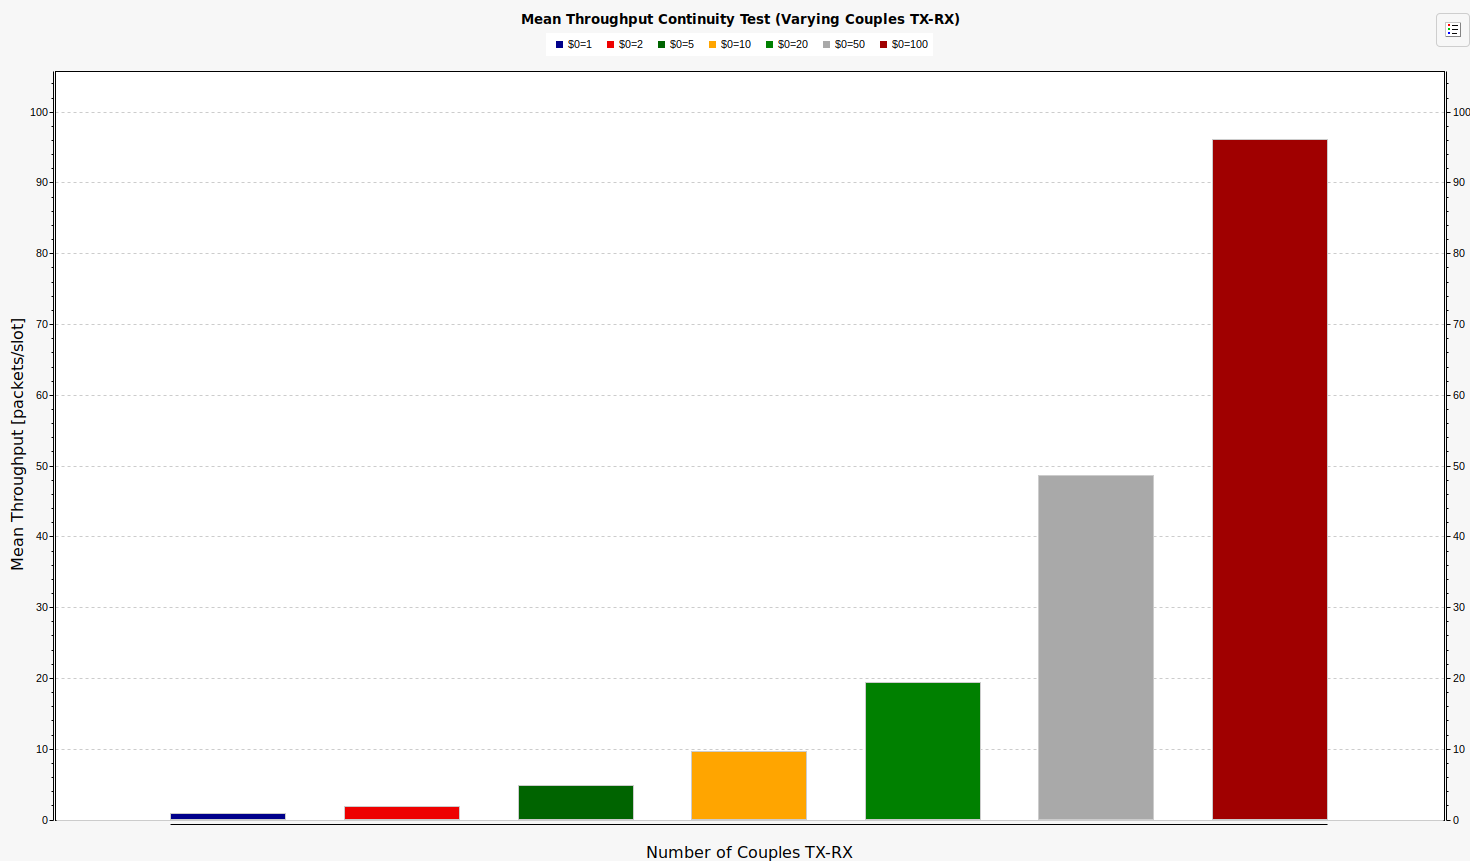
\includegraphics[width=\textwidth]{img/continuityTest_Throughput_TXRX_Varying.png}
		\caption{Continuity Test - Increasing Number of TX-RX (Main factors: \textbf{N} = 1, 2, 5, 10, 20, 100; \textbf{C} = 20000; $\dfrac{1}{\lambda}$ = 20 ms; $T_{slot}$ = 5ms; $p$ = 1)}
		\label {img: continuityTestThTXRX}
	\end{figure}
	\begin{figure}[H]
		\centering
		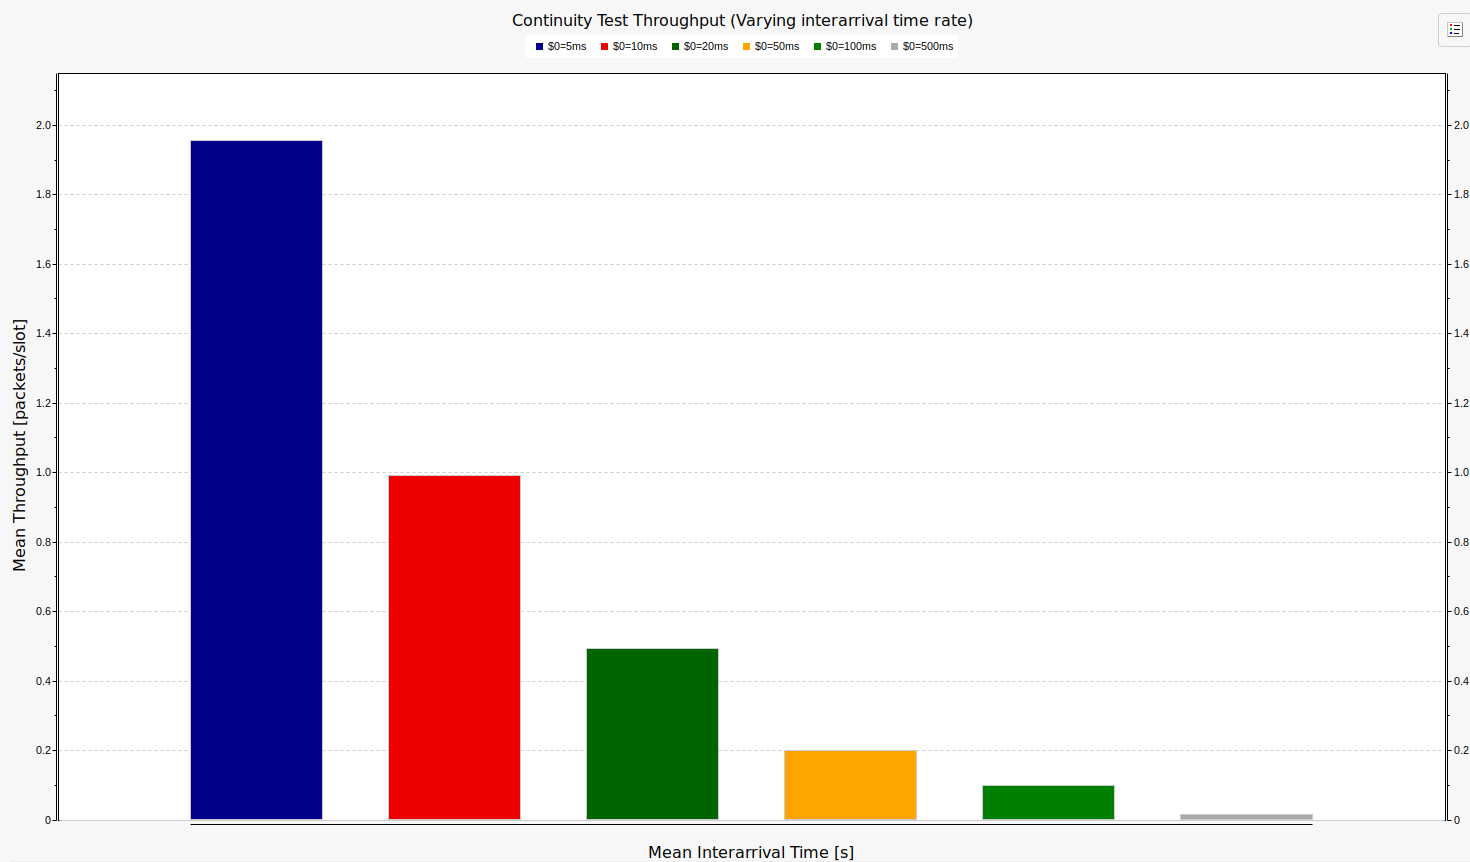
\includegraphics[width=\textwidth]{img/continuityTest_Throughput_IntTimeVarying.png}
		\caption{Continuity Test - Increasing Mean Inter-arrival Time (Main factors: \textbf{N} = 2; \textbf{C} = 20000; $\dfrac{1}{\lambda}$ = 5ms, 10ms, 20ms, 50ms, 100ms, 500ms; $T_{slot}$ = 5ms; $p$ = 1)}
		\label {img: continuityTestThLambda}
	\end{figure}
	\item \textbf{Mean Response Time}: By \textbf{Increasing N} ()the number of couples tx-rx), with low numbers of channels, a \textbf{increase on the mean response time is expected}. By increasing the transmission probability $p$ (with a low number of couples tx-rx) a decrease on the mean response time is expected due to more transmissions. The following results were obtained:
	\begin{figure}[H]
		\centering
		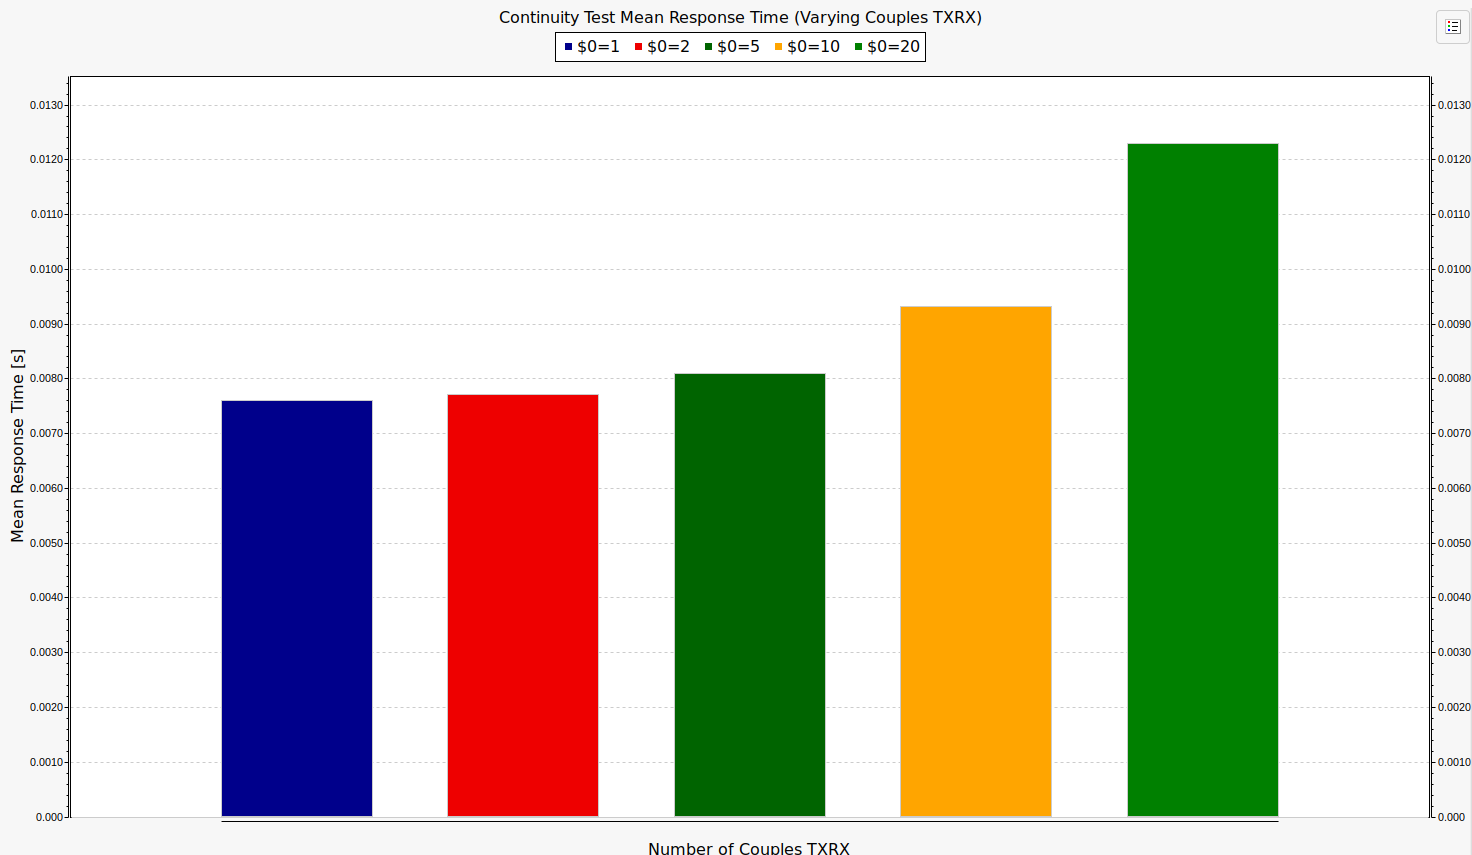
\includegraphics[width=\textwidth]{img/ContinuityTest_ResponseTIme_TXRXVarying}
		\caption{Continuity Test Mean Response Time- Increasing Number of TX-RX}
		\label {img: continuityTestTXRXResponse}
	\end{figure}
	\begin{figure}[H]
		\centering
		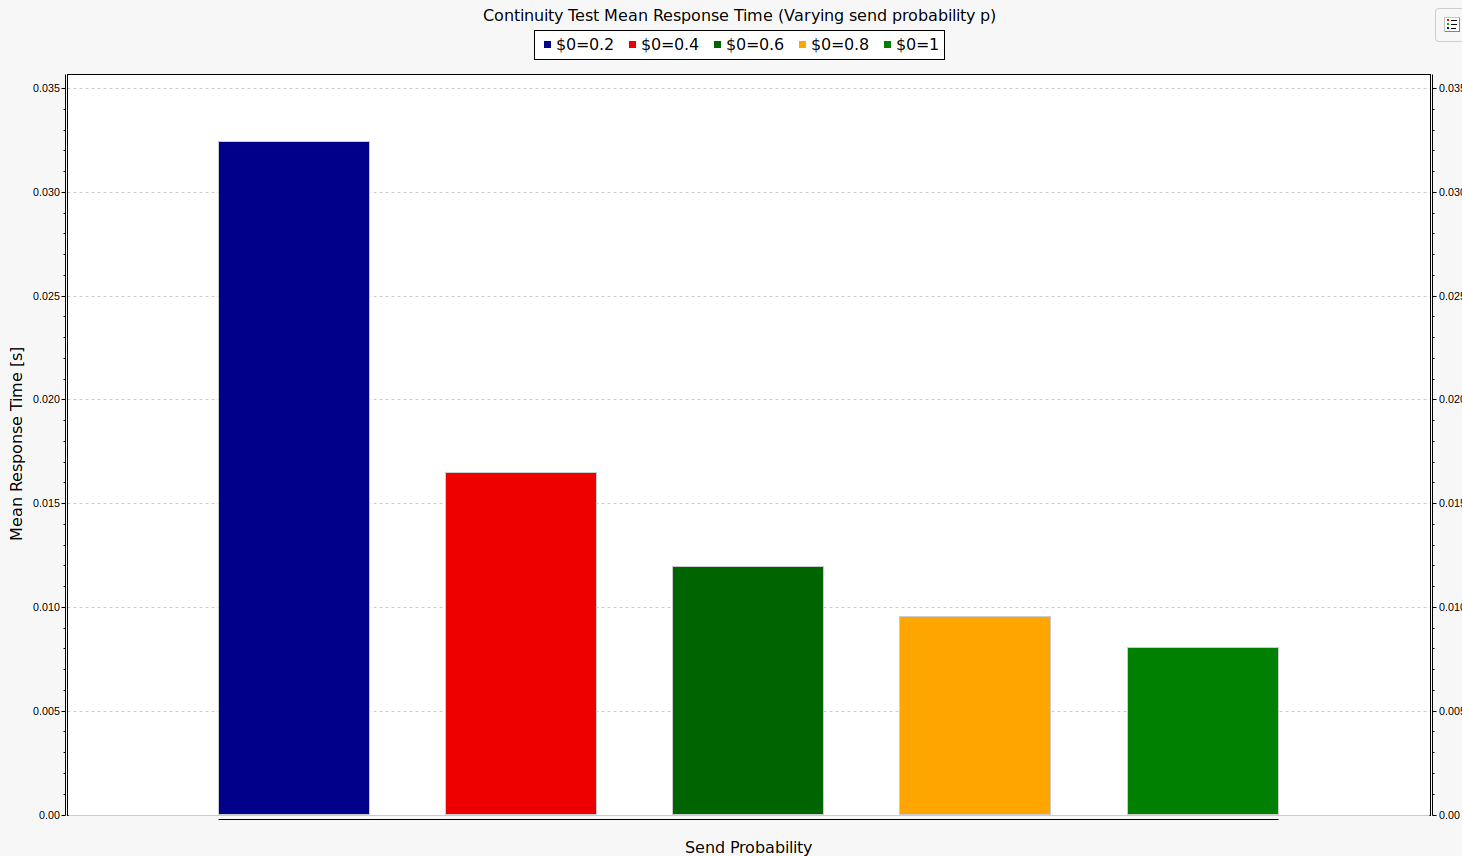
\includegraphics[width=\textwidth]{img/ContinuityTest_ResponseTIme_VaryingP.png}
		\caption{Continuity Test Mean Response Time- Increasing Sending Probability P(Main factors: \textbf{N} = 5; \textbf{C} = 4; $\dfrac{1}{\lambda}$ = 200ms; $T_{slot}$ = 5ms; $p$ = 0.2, 0.4, 0.6, 0.8, 1)}
		\label {img: continuityTestResponseLambda}
	\end{figure}
\end{itemize} 
\textbf{For the Mean Response Time was also checked the steady state reach} by just plotting that the relative vector stabilizes at some point (this was done in general to make conclusion with this KPI). Here an example for the varying of the Transmission Probability $p$:
\begin{figure}[H]
	\centering
	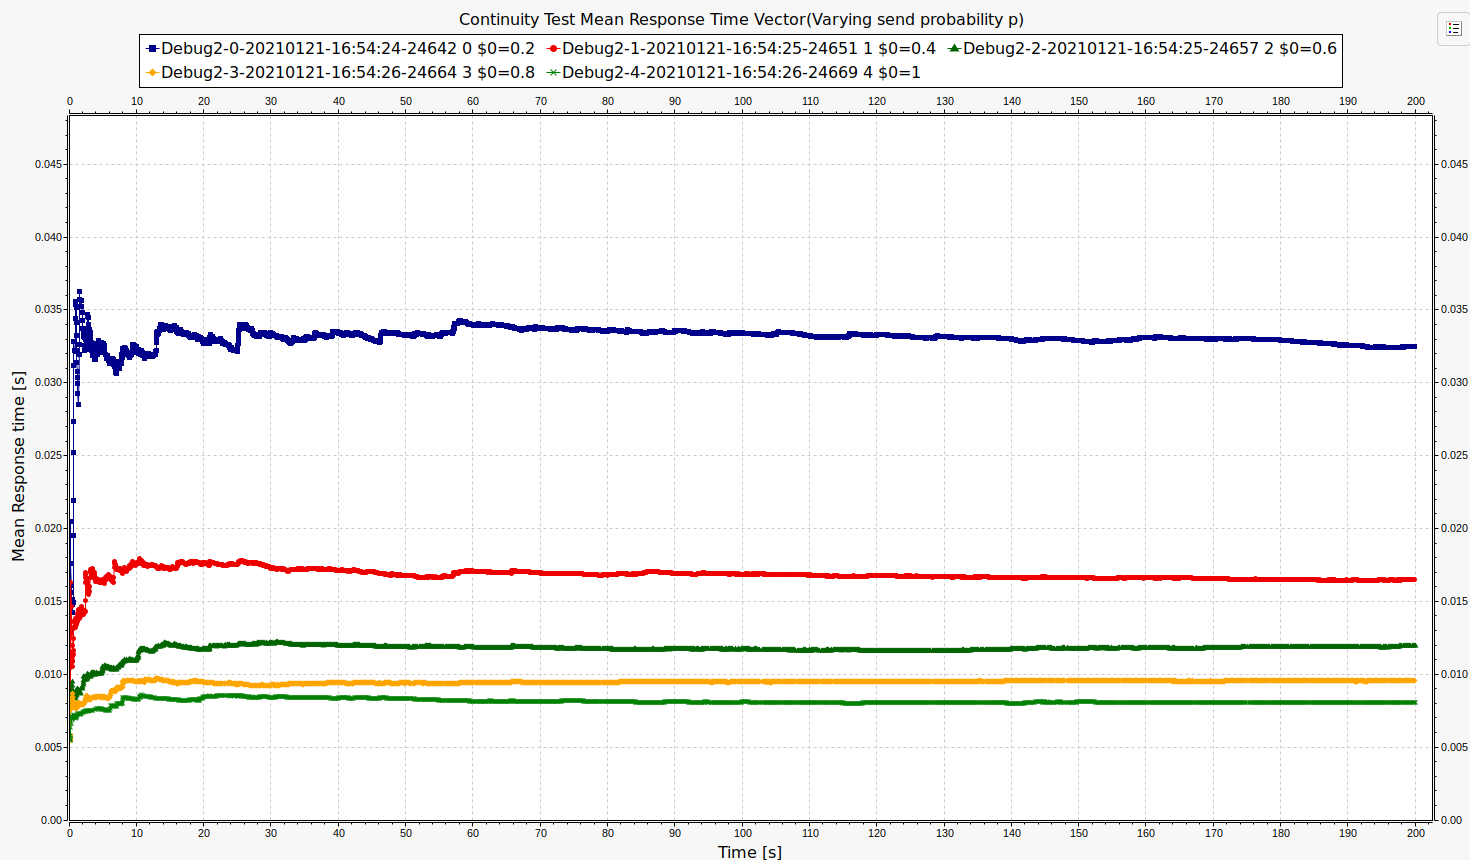
\includegraphics[width=0.8\textwidth]{img/ContinuityTest_ResponseTime_VectorP.png}
	\label {img: responseTimeConvergence}
\end{figure}
\subsection{Test Simulations with Binomial Model (1)}
This test simulation has been performed with the following parameters:
\paragraph{Parameters}
\begin{itemize}
	\item Number of couple tx-rx: 1
	\item Number of channels: 1
	\item Send probability: \$\{0.2, 0.4, 0.5, 0.6, 0.8\} ($p$)
	\item Mean inter-arrival time: 1s (deterministic) ($lambda$)
	\item Time slot size: 2s ($T_{slot}$)
	\item simulation-duration: 3600s ($T_{sim}$)
	\item repeat: 100
	\item seed-set: \$\{repetition\}
\end{itemize}
In this simplified context there are no collisions (only one couple) and the transmitter will have, for every slot, at least one packet to sent ($lambda < T_{slot}$). We can model this particular case as a repeated Bernoullian Experiment, in which a success event correspond to a successful packet sent. In this simplified model we can define X as the number of success in n repeated trials (in independent condition), so $X \sim Bin(n, p)$. For this reason the PMF is the following:
\begin{equation}
	p(i) = P\{X = i\} = \binom{n}{i} p^{i} (1-p)^{n-i}
\end{equation}
Where $n$ represents the number of repeated trials and $i$ the number of successes in those trials. With this distribution the mean and the variance are:
\begin{align*}
	E[X] = np \qquad     
	Var(X) = np(1-p)
\end{align*}
In our context we can state the following:
\begin{equation}
	n = \left \lfloor{\dfrac{T_{slot}}{T_{sim}}}\right \rfloor = 1800
\end{equation}
We would expect in the case of $p = 0.5$:
\begin{equation}
	E[X] = np = 900
\end{equation}
And the results after the run of 100 test simulation with different seeds, the following results are returned (with 95\% CI):
\begin{equation}
	\overline{X} \in [893.08, 901.94]
\end{equation}
Which is in line with our expectations. The latter computations have been repeated for different values of p and the following plot can sum up the results:

\begin{figure}[H]
	\centering
	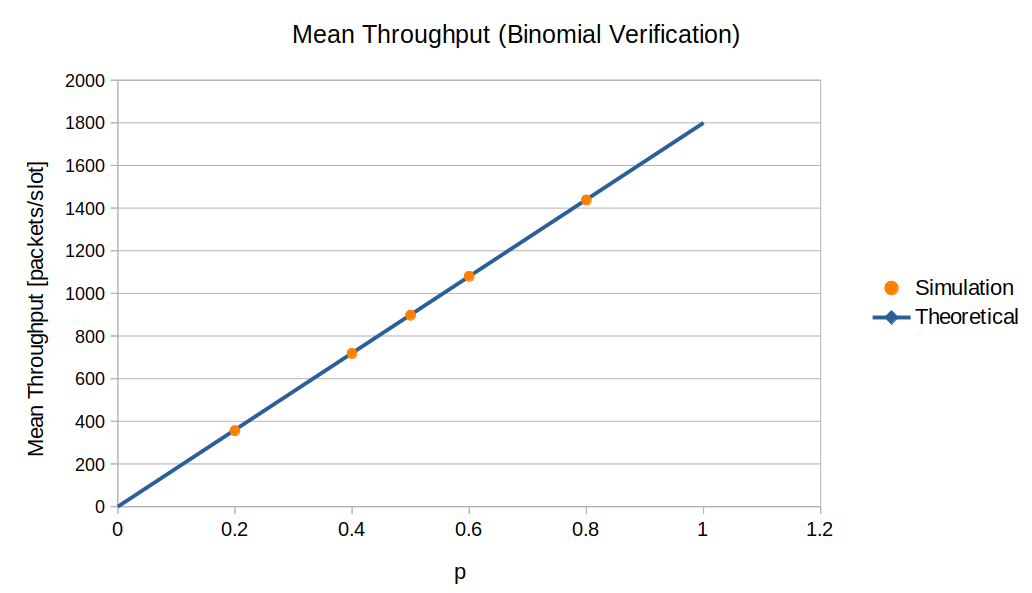
\includegraphics[width=0.9\textwidth]{img/plotTheoreticalMeanBinomial.png}
	\caption{Test Binomial Model}
\end{figure}

As we can see it is difficult to recognize the theoretical results with the results obtained with the test simulations and the Confidence Interval can be barely seen.

\subsection{Test Simulations with Collisions(2)}
This test simulation has been performed with the following parameters:
\paragraph{Parameters}
\begin{itemize}
	\item Number of couple tx-rx (N): \$\{2, 5, 10, 30\}
	\item Number of channels (C): 1
	\item Send probability: \$\{0.2, 0.4, 0.6, 0.8\} ($p$)
	\item Mean inter-arrival time: 1s (deterministic) ($lambda$)
	\item Time slot size: 2s ($T_{slot}$)
	\item simulation-duration: 3600s ($T_{sim}$)
	\item repeat: 40
	\item seed-set: \$\{repetition\}
	\item No Backoff in case of collision
\end{itemize}

\noindent The aim of this verification is to assess if the mean throughput is comparable with some equations that will be found even in the case of presence of collisions. \\

\noindent The probability of a successful sent in a particular timeslot, in this case, is the following:
\begin{equation}
	P\{" successful\ transmission"\} = P\{"only\ one\ tx\ transmit"\} = Np(1-p)^{N-1}
\end{equation}

Note that the above case is equal to the case without collisions.

By comparing the above formula with the results of the simulation the following results are obtained (95\% CI too small to be seen)
\begin{figure}[H]
	\centering
	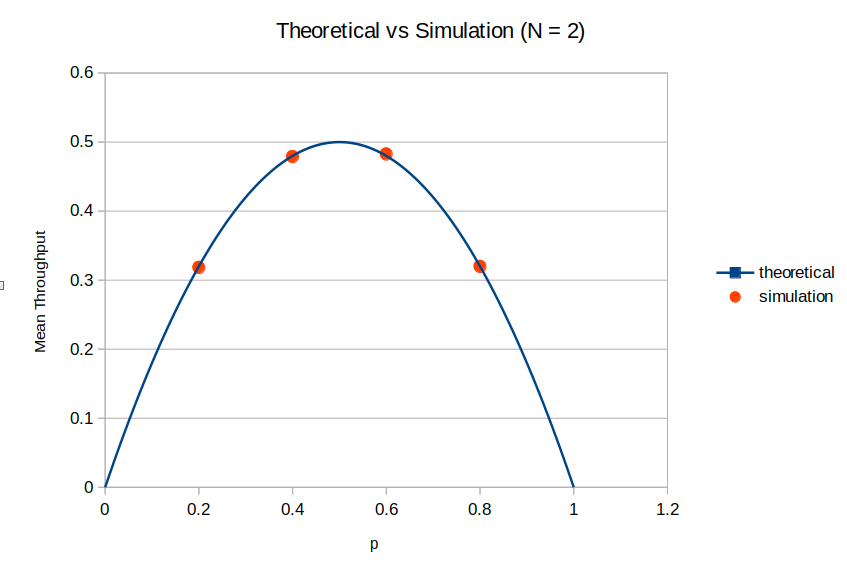
\includegraphics[width=\textwidth]{img/SecondVerificationN2.png}
\end{figure}
\begin{figure}[H]
	\centering
	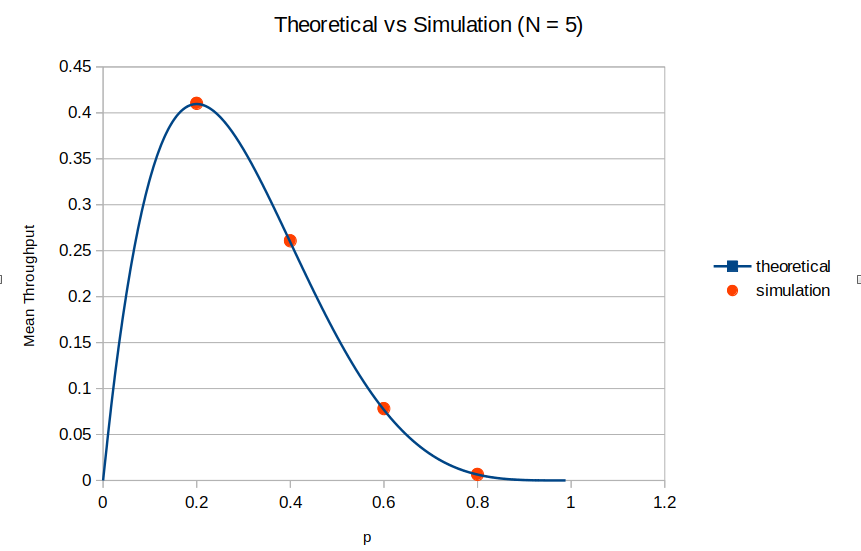
\includegraphics[width=\textwidth]{img/SecondVerificationN5.png}
\end{figure}
\begin{figure}[H]
	\centering
	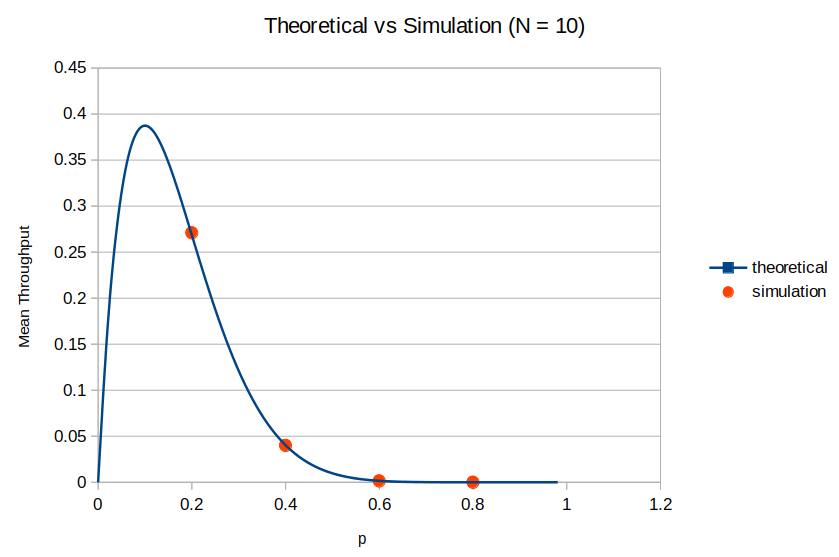
\includegraphics[width=\textwidth]{img/SecondVerificationN10.png}
\end{figure}
\begin{figure}[H]
	\centering
	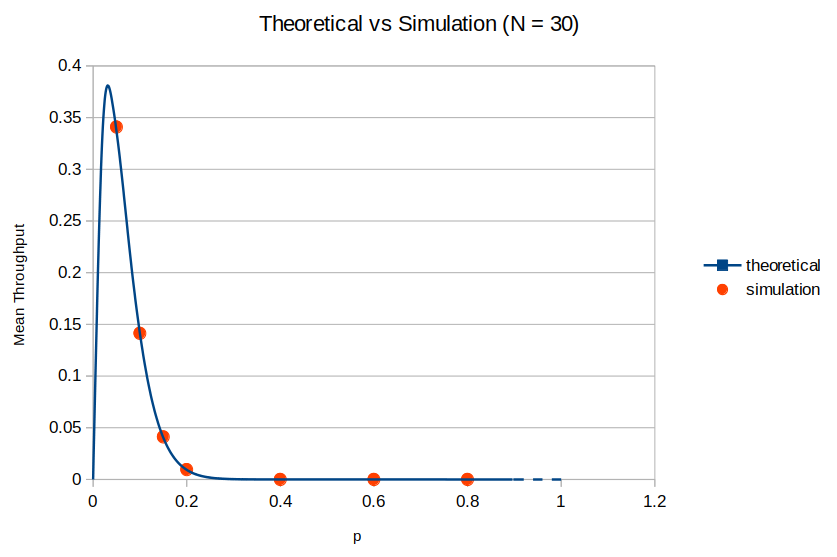
\includegraphics[width=\textwidth]{img/SecondVerificationN30.png}
\end{figure}

At this point we can state that a proper amount of verification of the implementation of the model has been carried out to make some simulation and gather some insight. Before doing so, an observation of the result can be carried out at this point: with a good number of couple tx-rx a huge sending probability (i.e. greater than 0.5) is pointless to obtain a high throughput. This result will be considered during the scenario calibration in the next chapter. 